\section{实验评估}
本节对 \gls{ismmdp} 和 \gls{immmdp} 进行分析。首先在 \Cref{subsec:setting_exp_mtd} 中描述实验设置，然后在 \Cref{subsec:results_mtd} 中展示和讨论结果。


\subsection{设置}
\label{subsec:setting_exp_mtd}
对于本节讨论的所有任务，我们运行 10 个随机种子并对结果取平均。

\subsubsection{任务}
\label{subsubsec:tasks_mtd}

\noindent\textbf{\gls{immmdp} 的 Pendulum 任务。}\indent 在此实验中，考虑本文已广泛研究的 Pendulum 任务。希望通过实验观察 \Cref{lem:same_distrib_psmmdp} 的结果。因此，研究在无延迟 \gls{mdp} 中使用 \gls{sac} 训练、在 \gls{immmdp} 中测试的同一策略 $\pi$ 的状态分布。这些状态分布将与无延迟环境中随机策略的状态分布进行比较。

\noindent\textbf{\gls{ismmdp} 的 Pendulum 任务。}\indent 然后，将实验重点放在 \gls{ismmdp} 上。在此第一个任务中，探索 Pendulum 环境中折扣期望回报的设置。研究延迟向量 $\boldsymbol\lambda$ 定义的延迟分布变化对智能体回报的影响。智能体的策略将使用 A-SAC 在从环境采样的 50,000 步中学习。

\noindent\textbf{迷宫（Maze）。}\indent 作为平均奖励设置的测试基准，考虑一个 3x3 网格世界\footnote{该环境可访问：\href{https://github.com/MattChanTK/gym-maze}{链接}。}，智能体必须学习从左上角的起始状态到达右下角的目标状态。网格内的墙壁使任务略有难度。智能体可以朝四个基本方向移动。当智能体撞到墙壁或环境边界时，它停留在同一单元格中。在此环境中，比较延迟向量 $\boldsymbol\lambda$ 的若干取值。具体地，对于 $\boldsymbol\lambda=(\lambda_0,\lambda_1)$，考虑 $\lambda_0,\lambda_1$ 在集合 $\{0,0.1,\dots,0.9\}$ 中的取值。特殊情况 $\boldsymbol\lambda=(1,0)$ 是无延迟情况，$\boldsymbol\lambda=(0,1)$ 对应常值 1 步延迟。由于目标是平均奖励，将考虑 UCRL2 算法并研究智能体的遗憾（见 \Cref{subsec:theoretical_rl}）。注意，即使在简单环境中，\gls{ismmdp} 情况下最优策略的计算也更加复杂。首先，即使底层 \gls{mdp} 是确定性的，过程的初始化也会在初始状态中引入随机性。其次，当延迟向量的权重不集中在单个元素上时，转移本身会进一步注入随机性。

\subsection{结果}
\label{subsec:results_mtd}

\noindent\textbf{\gls{immmdp} 的 Pendulum 任务。}\indent 我们在 \Cref{fig:state_distrib_pendulum_mtd} 中报告三个过程的状态分布。这些分布通过运行 Pendulum 环境的多个回合获得。显然，无延迟 \gls{sac} 策略在无延迟 \gls{mdp} 和 \gls{psmmdp} 上产生相似的状态分布。该分布与随机策略的状态分布差异很大。可以观察到一条最内层抛物线，其中仅出现来自无延迟过程的状态。低速度和小幅度的状态典型地出现在过程的初始步骤中，延迟过程未观察到此类状态可能归因于延迟初始化偏移（见 \Cref{subsec:delay_init}）。环境中首个随机采样的动作赋予了初始速度或角度，使智能体从不同位置开始。这并不否定我们的理论，因为这些初始状态对于接近最优策略的 \gls{sac} 来说是瞬态的。

\begin{figure}[t]
    \centering
    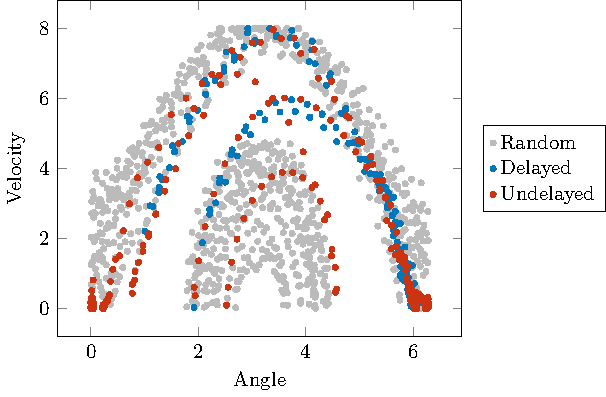
\includegraphics[labelmtdstates=statesdistribmtdpendulum]{img/thesis_plots_chapter_mtd_states.pdf}
    \caption{使用 \gls{sac} 获得的策略在无延迟 Pendulum 环境及其延迟 \gls{psmmdp} 对应环境中测试的状态分布比较。
    状态由两个元素组成：速度和摆杆角度。
    添加无延迟环境中随机策略的状态分布作为比较。}
    \label{fig:state_distrib_pendulum_mtd}
\end{figure}


\noindent\textbf{\gls{ismmdp} 的 Pendulum 任务。}\indent \Cref{fig:pendulum_mtd} 展示了不同延迟向量取值获得的回报。随着延迟分布开始向较长延迟偏移，回报开始下降，这与 \Cref{conj:delay_cumulativ_distrib} 的预期一致。更仔细地观察结果，当延迟向量分布在两个连续的 $\lambda$ 值上时（$(\lambda_i=0.5,\lambda_{i+1}=0.5)$），性能通常低于 $(\lambda_{i+1}=1)$，尽管差异不显著。这可能与 \Cref{conj:delay_cumulativ_distrib} 相悖，但可能仅由学习问题导致。实际上，用于训练 A-SAC 的样本数对所有延迟都是固定的，但 $(\lambda_i=0.5,\lambda_{i+1}=0.5)$ 类型的延迟在转移概率中注入了更多随机性，可能使最优策略的学习更加困难。

\begin{figure}[t]
    \centering
    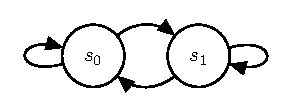
\includegraphics[labelmtd=pendulummtd]{img/thesis_plots_mtd.pdf}
    \caption{A-SAC 在 Pendulum 环境中针对不同延迟向量 $\boldsymbol\lambda$ 取值测试的回报演变。
    注意无延迟（$\lambda_0=1$）和常值 $\delay$-延迟环境（$\lambda_{\delay}=1$）的特殊取值。}
    \label{fig:pendulum_mtd}
\end{figure}

\noindent\textbf{迷宫。}\indent \Cref{fig:grid_world_ucrl} 报告了结果。这里同样可以更清楚地观察到延迟分布偏移的影响。随着延迟分布在较长延迟上分配更多权重，遗憾增加。有趣的是，常值延迟情况（$\boldsymbol\lambda_0=1$ 和 $\boldsymbol\lambda_1=1$）与其他延迟向量之间似乎存在差距。尽管按累积分布排列，随机延迟的遗憾是聚集的，且显著偏离常值延迟的遗憾。

\begin{figure}[t]
    \centering
    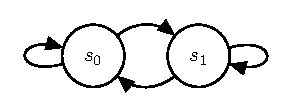
\includegraphics[labelmtd=gridworld]{img/thesis_plots_mtd.pdf}
    \caption{
    UCRL2 在迷宫环境中针对不同延迟向量 $\boldsymbol\lambda$ 取值测试的遗憾演变。
    注意无延迟（$\boldsymbol\lambda=(1,0)$）和常值 1 步延迟（$\boldsymbol\lambda=(0,1)$）过程的特殊情况。}
    \label{fig:grid_world_ucrl}
\end{figure}